\definecolor{gray}{rgb}{0.4,0.4,0.4}
\definecolor{darkblue}{rgb}{0.0,0.0,0.6}
\definecolor{cyan}{rgb}{0.0,0.6,0.6}

\lstset{
  basicstyle=\ttfamily,
  columns=fullflexible,
  showstringspaces=flase,
  commentstyle=\color{gray}\upshape
}

\lstdefinelanguage{XML}
{
  morestring=[b]",
  morestring=[s]{>}{<},
  morecomment=[s]{<?}{?>},
  stringstyle=\color{black},
  identifierstyle=\color{darkblue},
  keywordstyle=\color{cyan},
  morekeywords={xmlns,version,type}% list your attributes here
}


% CREATED BY DAVID FRISK, 2015
\chapter{Methods}\label{ch_3}
In this chapter, we will thoroughly analyse the ways with which the three processing stages which were presented in the previous units, were implemented.\\
\\
In order to describe in the best possible way the process that was followed, a detailed description of the dataset which was used will be given, as well as of the features that characterise it. Then, we will describe the relational database model which we used to store the information from the texts (dataset). Finally, for each one of the process stages, we will describe the methodology with which each matter was approached.

\section{Preparing the Dataset}\label{31_ref}
In this part of the methodology, the features of the used dataset (\ref{311_ref}) will be described in detail. Some information on the way of choosing data (\ref{312_ref}) will be described as well. Next, the way of data mining from the Greek Open Government platform\footnote{\url{http://www.opengov.gr}} (\ref{313_ref}) and finally, the Entity-Relationship Model (\ref{314_ref}) of the database which was used to store the data will also be described.

\subsection{Dataset} \label{311_ref}
As already mentioned, the data that were used have been taken from the Greek Open Government platform, which constitutes a platform of electronic consultation of citizens on texts, more specifically on laws and decrees that the Greek Government issues. These data are open and accessible to everyone.\\
\\
In this section, the basic features of the studied texts will be described. The reason why this section comes first in this part of the methodology, is that the very nature of these texts (they are basically users' comments to the on-line service), created many problems in their analysis.\\
\\
As it has already been mentioned, the texts that were studied feature several oddities, some of which made the process of analysing them difficult.\\

\begin{itemize}
  \item Initially, the first that we can notice is that the length of the texts is 	relatively short. To be precise, it is rare for them to be longer than 3000 characters (approximately 200 words, 80\% of the texts). The length of the text did not affect all the stages of the analysis. The biggest difficulty appeared in the effort to extract the degree of the writer's agreement with the initial text (more details will be given later).\\
  
  \item A second remark is the fact that the texts that were studied do not constitute an official text. In particular, the texts contain users' comments in an on-line service, and many of them contain spelling, grammatical or other errors that hinder their analysis.. This created many difficulties in the studying of these comments. The first difficulty had to do with the tools needed in order to conduct the overall analysis of each text. The basic idea was that the tools had to be tolerant when it came to errors, at least up to a degree.\\
\\
Some very usual errors are:

  	\begin{enumerate}
  	\item spelling errors
  	\item absence of some letters in a word
  	\item letter transposition in a word
  	\item use only of capital letters
  	\item absence of punctuation
  	\item wrong sentence separation (there was no gap after the dot)
	\end{enumerate}

  \item As it was mentioned the commentaries do not constitute an official text, so there are many times when syntactical structure errors are spotted. This problem is directly connected to the use of POS-Tagger for the syntactic analysis (parsing) of texts. This issue affects, to some degree, the extrapolation of arguments and of proposals and counter proposals that the user makes.\\
  
  \item Another feature is that the texts are entirely in Greek. This problem is more 	serious, because there are no tools which we needed at some point of the analysis, that support the Greek Language. Subsequently, as we will see later on, there was the need to resort to some compromising solutions.\\
  
  \item One last issue that is worth mentioning, which constitutes a more qualitative feature, at least in the whole of texts that were studied, is the fact that the majority of users who wrote a comment are ``annoyed''. This ``annoyance'' stems from the fact that the texts that are under discussion contain laws and presidential decrees most of which, lead to a decrease in public spending towards the citizens. This ``annoyance'' is noted almost in the entire dataset that we studied. The problem is that the texts in which the writers agree with the initial text are limited. As a result, this issue complicates the process of detecting, if the writer agrees with the initial text. Also another serious problem is that the ``annoyance'' causes the users to make several kind of mistakes (such as grammatical, syntactical etc.).
\end{itemize}


\subsection{Choosing the Set of Documents}\label{312_ref}
To continue the process, we manually chose five different bills that contained a significant amount of users' replies. Afterwards, we selected a few, trying to eliminate the replies that we did not want to process. For example:\\

\begin{itemize}

	\item replies that only contained one sentence
	\item replies in greeklish\\

\end{itemize}

Next, we limited the dataset so as to contain a number of approximately two hundred replies. This total is the final dataset that was studied and on which the conclusions for all the processing stages were based.

\subsection{Finalizing the Dataset}\label{313_ref}
The last step for the creation of the final dataset was the data mining from the Greek Open Government platform\footnote{\url{http://www.opengov.gr}} (the website for public consultation on laws). This process was  simple enough, since the service provides the users with the option to locally store all the comments that have been posted for each law or decree. The data were in excel file format, providing for each comment the following meta-data:\\

\begin{itemize}

	\item the Law Article which was commented
	\item an id for each comment
	\item the name of the user-commenter
	\item the date\\

\end{itemize}

These data were later stored in the database which was created for the storage of data that were collected in all the stages of processing.

\subsection{Database}\label{314_ref}
In order to store the final database with the selected bills and comments, an MySQL\footnote{\url{https://www.mysql.com}} Database was created, whose Entity-Relation Model\footnote{\url{http://www.aw-bc.com/info/riccardi/database/Riccardi_ch4.PDF}} can be presented in the following layout.
\newpage
\begin{figure}[H]
\centering
\includegraphics[width=1.05\linewidth]{figure/ER.pdf}
\caption{Entity - Relation Model}
\end{figure}

In the above layout, we can see the Entity-Relation Model that was used for storing data. Next, the tables  which appeared in the above diagram will be described in detail:\\

\begin{itemize}

	\item \textbf{opngv\textunderscore comment:} It is used to store texts which have been extracted from the public consultation web page and more precisely, each commentary is stored in the raw called ''comment'' of the ``opengov\_ comment'' table. The rest of the elements of this text are used to store some meta data of the texts (e.g. law name/number, name of the author, date).
	\item \textbf{opngv\textunderscore sentiment:} This table is used to store the information that is extracted after the completion of the process. More precisely, in the ``Sentiment'' field, the information that is stored defines whether a user's text/comment is negative or positive,
	\item \textbf{opngv\textunderscore sentence:} This table is used to store sentences that make up the text. In the ``sentence'' field, each sentence of the commentary is stored. The word "sentence" used with the literal significance so the separation of the text is done by using POS-Tagger.
	\item \textbf{opngv\textunderscore argument:} It contains the values of the argument markers for each sentence. Each variable of this table is explained in unit (\ref{321_ref}).
	\item \textbf{opngv\textunderscore suggestions:} Respectively with the ``opngv\_ argument'' field, this field contains the suggestion markers.
	\item \textbf{opngv\textunderscore trainset:} This table contains data which declare whether a sentence is an Argument or a Suggestion. These data are stored in the boolean variables of the table (argument, suggestion). The data of this table make up the train set that is used for machine learning. More precisely, the train set comes up by combining the ``opngv\textunderscore argument'' and the ``opngv\textunderscore suggestion'' tables with this table.\\

\end{itemize}

In all the table,the primary keys have been marked with bold.

\subsection{Building a Trainset}\label{315_ref}
One last element that deals with the chapter on dataset, is characterising a total of sentences if each one of them contains an Argument or a Suggestion. We should note here that sentence separation will be analysed thoroughly later (\ref{3221_ref}). The Train set that we created, as we will see in the chapters that follow, is needed so that the machine learning algorithms can be trained, as well as to achieve a better evaluation. The set of sentences that was created contains approximately one thousand sentences.


\section{Argument Extraction}\label{32_ref}
At this point, the process with which the Argument Extraction was carried out on the whole of the texts will be described. The process is based on three stages:\\
\\
\begin{itemize}

	\item Selecting Argument Markers (\ref{321_ref}).
	\item POS-Tagging the set of documents (\ref{322_ref}).
	\item Applying machine learning  to the Argument Markers (\ref{323_ref}).\\

\end{itemize}

\begin{figure}[H]
\centering
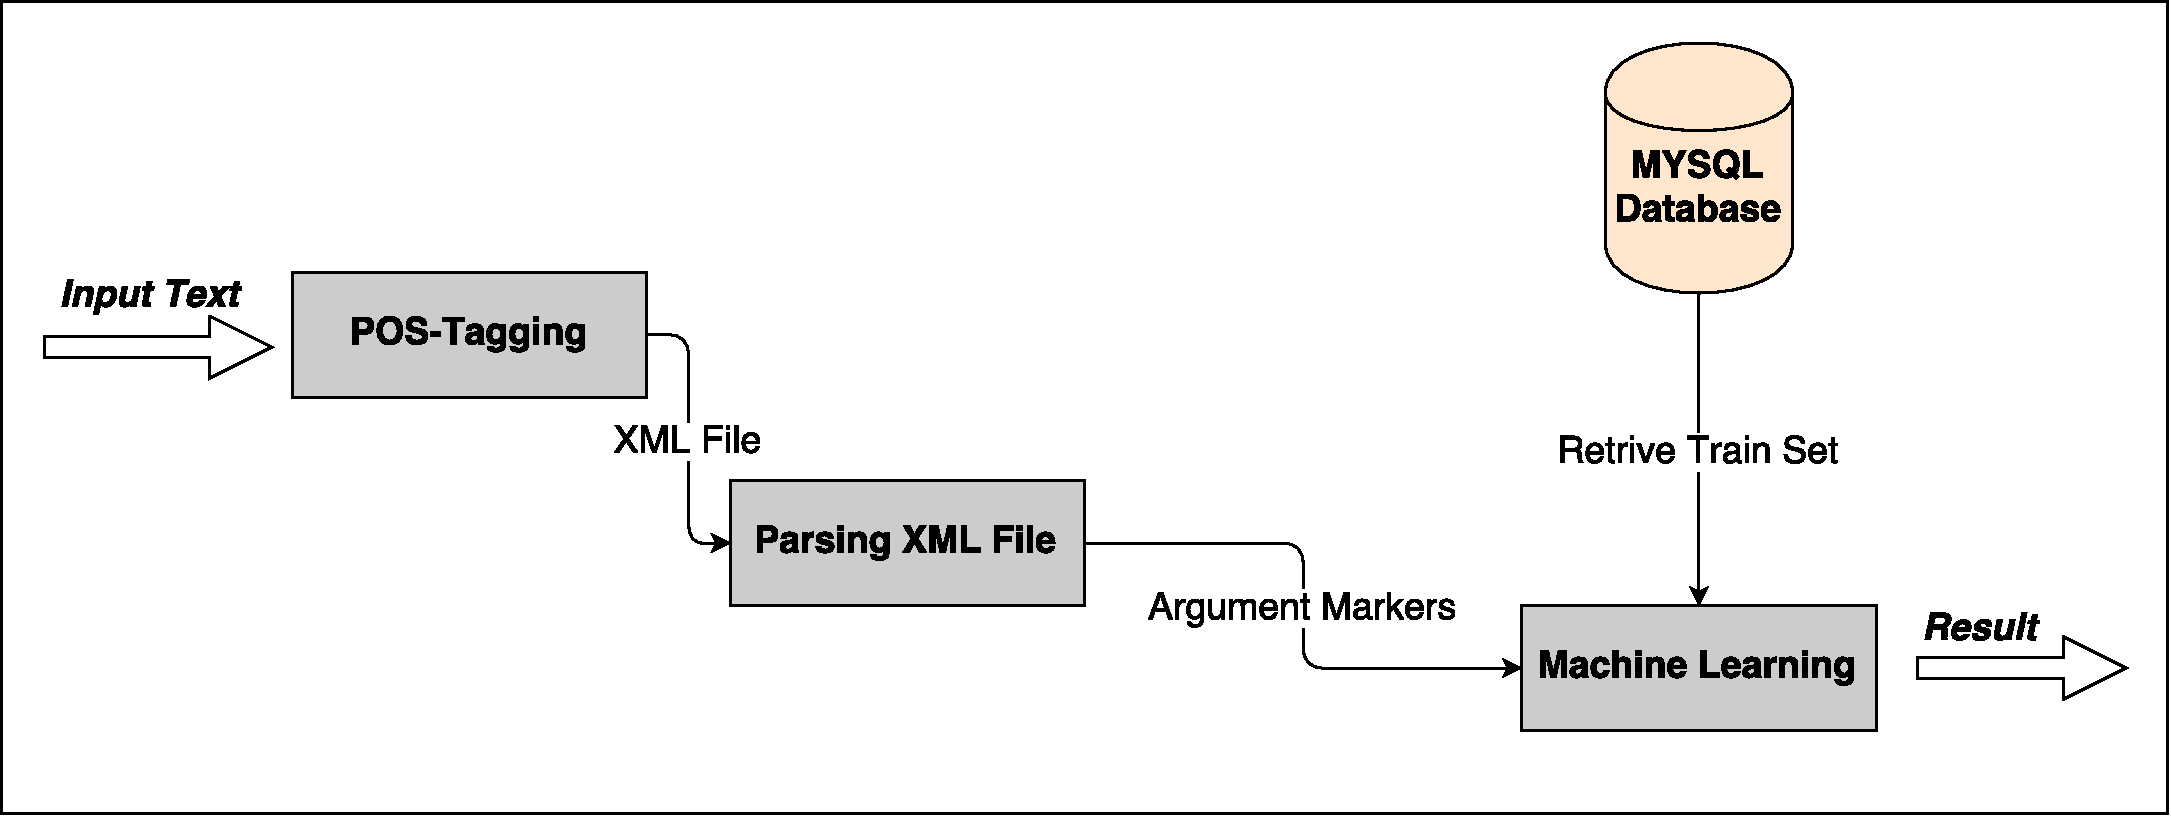
\includegraphics[width=1\linewidth]{figure/methods/argument_extraction.pdf}
\caption{Argument Extraction Process}
\end{figure}

Each one of the three stages will be explained right away.

\subsection{Selecting Argument Markers}\label{321_ref}
This step, in essence, constitutes the selection process of certain ``criteria'' - ``Argument Markers'' that will help us define what an argument is. Essentially, this process constituted the hardest part in the whole Argument Extraction stage.\\
\\
For this step, we decided to use Machine Learning techniques, an approach that is popular in the related literature (\ref{321_ref}). In particular, our approach consists in defining some parameters which will define with a relative clarity whether a sentence is an argument or not.\\
\\
But before we get in the process of searching for these variables, we had one more difficulty to face. Even though it sounds relatively easy to recognise the arguments in a text, in reality it was a rather difficult process. In experiments with human users, it turned out that there was great difficulty, even among humans, to agree on whether a sentence contains an argument or not. To address this problem, we formulated the following definition:\\
\\
\textit{Sentence is likely to contain an argument if it contains the following markers:\\}
\begin{itemize}

	\item \textit{The sentence provides a context clue from which we can interpret that the writer expresses an opinion}.
	\item \textit{The sentence is explanatory, which means that the writer wants either to further explain or support an opinion.\\}
	
\end{itemize}

If there is any of the above markers in a sentence, then this sentence can be characterised as an argument (Argumentative sentence). Even with the above two conventions, in some cases it is still difficult to determine whether a sentence is an argument. More precisely, another convention has been set, with which we made an effort to define that the interrogative sentences are not congaing any arguments. The reason is that usually, interrogative sentences are likely to express sarcasm. In our dataset this was actually very usual.\\
\\
Having set the above conventions, we studied a total of Argumentative Sentences, in order to be able to track down ``Argument Markers''. In essence, we looked for parts of speech (for example the number of verbs, number of adjectives and more), as well as other variables that often appear in this type of sentences. These variables were to be used in the next steps and especially in the step where the ``Machine Learning'' process is applied\\
\\
From the study that was conducted, also combining Related work, we ended up with the following variables:\\
\\
\begin{itemize}

	\item \textbf{Number of Verbs:} In many studies which have been conducted in the past, it was noted that verbs are closely linked to arguments. To be precise, verbs express action. Another characteristic is that verbs syntactically compose a sentence or, a little more arbitrarily, verbs enrich a sentence. Consequently, it was noted that the sentences which contain arguments usually have a larger number of verbs.
	\item \textbf{Number of Verbs in Passive Voice:} The bibliography that we had available mentions that usually the verbs that are in the passive voice are used when someone claims something concerning a particular matter. In our dataset this was not so clear. However, in the measurements done, we noted that most sentences containing an argument also contain, to a great extent, verbs that are in the passive voice.
	\item \textbf{Key Words:} This variable refers to the number of words that were traced in a group of words that we created. This group contains words that are used when someone tries to explain or support an opinion. For example, in this group there are the words  consider, believe, admit, suppose, think, must, consequently, since, until, because, namely.
	\item \textbf{Number of Connective Words:} This variable counts the number of linking words that were found in a sentence. In essence, this number has a direct relation to the next variable which shows the total number of words. The idea of counting the length of a sentence lies to the fact that usually, longer sentences are more likely to contain arguments. Especially when the studied dataset contains texts with arguments and political discussion.
	\item \textbf{Total Number of Words:} similar to the previous variable.
	\item \textbf{Average Number of Letters in a Word:} This variable came up from the bibliography that we had available. It has been noted that this variable, especially in texts that contain political discussion, can help in a significant way to track arguments.
	\item \textbf{Number of Adjectives:} It is the number of arguments that were found in a sentence. The logic behind this variable is the same  with  the ``Number of Verbs'' variable logic.
	\item \textbf{Number of Adverbs:} It came up after studying the reference and it states the number of adverbs in a sentence.
	\item \textbf{Number of Nouns:} The role of this variable is equivalent to the ``Number of Adjectives'' variable.
	\item \textbf{A Boolean Variable that States Whether a Sentence is Interrogative:} The need for this variable was explained thoroughly above.

\end{itemize}

\subsection{POS-Tagging}\label{322_ref}
In this part we will analyse the second step in the process of argument extraction from a text. Unlike the previous step (\ref{321_ref}), the execution of this step is essential for every new step we wish to analyse.\\
\\
As it has already been mentioned above (\ref{22_ref}), the POS-Tagging procedure has as goal to analyse the grammar of the text, as well as to extract an output which will contain a recognition of what part of speech each word is. Clearly, this process is very important for Argument Extraction because it constitutes the way with which all parts of speech will be detected.

\subsubsection{POS-Tagger}\label{3221_ref}
In this Thesis, ``ILSP POS-Tagger\footnote{\url{http://nlp.ilsp.gr/soaplab2-axis/}}'' was used, which was created by the ``Institute of Language and Speech processing\footnote{\url{http://www.ilsp.gr/en}}''. Also the POS-Tagger is used in order to split the text into sentences. This feature appears in the next section (\ref{3222_ref}) in which we can see the output that the Tagger produces.

\subsubsection{POS-Tagger Output}\label{3222_ref}
From the outputs supported by POS-Tagger that we had available, we have chosen the ``xceslemma'' option. With this option beyond POS-Tagging, Lemmatization can also be accomplished. We will need the latter in the next unit that we are going to study. The output given is in XML format. An example can be seen below:\\
%\newpage
\lstset{language=XML,
  morekeywords={id,word,lemma,tag}
}
%\greektext
\begin{lstlisting}[frame=single, basicstyle=\small]
<?xml version='1.0' encoding='UTF-8'?>
<cesDoc xmlns="http://www.xces.org/schema/2003" version="0.4">
  <text>
    <body>
      <p id="p1">
        <s id="s1">
          <t id="t1" word="..." tag="AtDfNeSgNm" lemma="..."/>
          <t id="t2" word="..." tag="RgFwOr" lemma="..."/>
          <t id="t3" word="..." tag="PnReNe03SgNmXx" lemma="..."/>
          <t id="t4" word="..." tag="VbMnIdPr03SgXxIpPvXx" lemma="..."/>
          <t id="t5" word="..." tag="VbMnIdPr03SgXxIpPvXx" lemma="..."/>
          <t id="t6" word="..." tag="AsPpSp" lemma="..."/>
          <t id="t7" word="..." tag="NoCmFeSgAc" lemma="..."/>
          <t id="t8" word="..." tag="RgFwOr" lemma="..."/>
          <t id="t9" word="..." tag="PTERM_P" lemma="..."/>
        </s>
      </p>
    </body>
  </text>
</cesDoc>
\end{lstlisting}
%\latintext
The text that was given as input was \textit{``The output which is given is in XML format''}. We note that for every word of the text, the following information is given:\\

\begin{itemize}
	
	\item \textbf{Id:} an auto increment identifier given in every word of the text
	\item \textbf{Word:} the initial word of the text
	\item \textbf{Tag:} the Grammar concerning the particular word. For example, verbs start with ``Vb'' and nouns with ``No''. The whole tagset can be found here:\\ \url{http://nlp.ilsp.gr/nlp/tagset_examples/tagset_en/}.
	\item \textbf{Lemma:} it is the dictionary entry of each word. For example, we note that the verb ``given'' has ``give'' as its lemma.\\

\end{itemize}

Although we gave a link to the tagset of the POS-Tagger, it is important at this point to give a brief explanation. For example, the tag ``VbIsIdPr03SgXxIpAvXx'' means:\\

\begin{itemize}

	\item \textbf{Vb:} verb
	\item \textbf{Is:} Impersonal
	\item \textbf{Id:} Indicative
	\item \textbf{Pr:} Present
	\item \textbf{03:} Third Person
	\item \textbf{Sg:} Singular
	\item \textbf{Xx:} Gender, No Value
	\item \textbf{Ip:} Imperfective
	\item \textbf{Av:} Active
	\item \textbf{Xx:} Case, No Value

\end{itemize}

\subsubsection{Parsing XML File}\label{3223_ref}
For the operation and data extraction from the XML file, DOM (Document Object Model\footnote{\url{http://www.w3.org/DOM/}}) was used, which is a platform for the representation and the interaction with objects in XML files. In this platform, the nodes of each file are organised in a tree form called the DOM tree. The objects in the DOM tree can be operated using the methods for objects. DOM's public interface is determined in Application Programming Interface.

\subsubsection{Uploading to Database}\label{3224_ref}
Finally, the data from the Parsing of XML file (\ref{3223_ref}) are stored in the Database and more precisely in the ``opngv\textunderscore argument'' table. For storing, the following Query is used:\\
\lstset{language=SQL}
\begin{lstlisting}[frame=single, basicstyle=\small]
INSERT INTO opngv_argument VALUES (values..)
\end{lstlisting}


\subsection{Apply Machine Learning}\label{323_ref}
The last stage for argument retrieval consists of the application of a Machine Learning process. In order for this process to be accomplished, a train set and a test set should have been clearly set.

%\newpage
\subsubsection{Selecting Train and Test Set}\label{3231_ref}
In this case in point, the train set is stored in the Data Base. More precisely, the train set retrieval from the Database is done with the following query:\\
%\newpage
\lstset{language=SQL}
\begin{lstlisting}[frame=single, basicstyle=\small]
SELECT
	opngv_argument.verbs,
	opngv_argument.pv_verbs,
	opngv_argument.cue_words,
	opngv_argument.connective_words,
	opngv_argument.total_words,
	opngv_argument.word_mean_length,
	opngv_argument.adjective,
	opngv_argument.adverbs,
	opngv_argument.noons,
	opngv_argument.question,
	opngv_trainset.Argument
FROM
	opngv_sentence
	INNER JOIN opngv_argument
		ON opngv_sentence.comment_id = opngv_argument.comment_id
	 	AND opngv_sentence.sentence_id = opngv_argument.sentence_id
	INNER JOIN opngv_trainset
	 	ON opngv_sentence.comment_id = opngv_trainset.comment_id
	 	AND opngv_sentence.sentence_id = opngv_trainset.sentence_id
\end{lstlisting}
On the other hand the test set constitutes the total of the sentences of a text, which we wish to analyse. In essence, to make it clearer, two tables, which contain the same columns, are created every time. The train set table contains the data as described in units (\ref{315_ref}) and (\ref{321_ref}). The second table (test set), contains the data that came up from the process that was described in unit (\ref{322_ref}) for new texts.

\subsubsection{Machine Learning Process}\label{3232_ref}
For the application of a Machine Learning Process, the Weka Framework ``Weka 3: Data Mining Software in Java\footnote{\url{http://www.cs.waikato.ac.nz/ml/weka/}}'' was used.\\
\\
\textit{“Weka is a collection of machine learning algorithms for data mining tasks. The algorithms can either be applied directly to a dataset or called from your own Java code. Weka contains tools for data pre-processing, classification, regression, clustering, association rules, and visualization. It is also well-suited for developing new machine learning schemes.”}

\subsubsection{Machine Learning Algorithms}\label{3233_ref}
To verify the accuracy of the Train set, we tried many algorithms:\\

\begin{itemize}

	\item Logistic Regression\footnote{\url{http://eu.wiley.com/WileyCDA/WileyTitle/productCd-0470582472.html}}
	\item Native Bayes\footnote{\url{http://nlp.stanford.edu/IR-book/html/htmledition/naive-bayes-text-classification-1.html}}
	\item Support Vector Machines\footnote{\url{http://www.support-vector.net/}}
	\item Random Forest\footnote{\url{http://link.springer.com/chapter/10.10072F978-0-387-84858-7_15}}\\

\end{itemize}
The results will be analysed in the following units.

\section{Suggestion Extraction}\label{33_ref}
At this section we will describe the procedure that we followed in order to achieve the Suggestion Extraction. The Procedure has five steps:\\
\begin{itemize}

	\item Selecting Suggestion Markers (\ref{331_ref})
	\item POS-Tagging \& Lemmatization the set of Documents (\ref{332_ref})
	\item Apply Information Retrieval Methods in order to find the suggestions (\ref{333_ref}) 
	\item Adding additional features for the optimization of\\Machine Learning Process (\ref{334_ref})
	\item Apply Machine Learning (\ref{335_ref})\\

\end{itemize}

\begin{figure}[H]
\centering
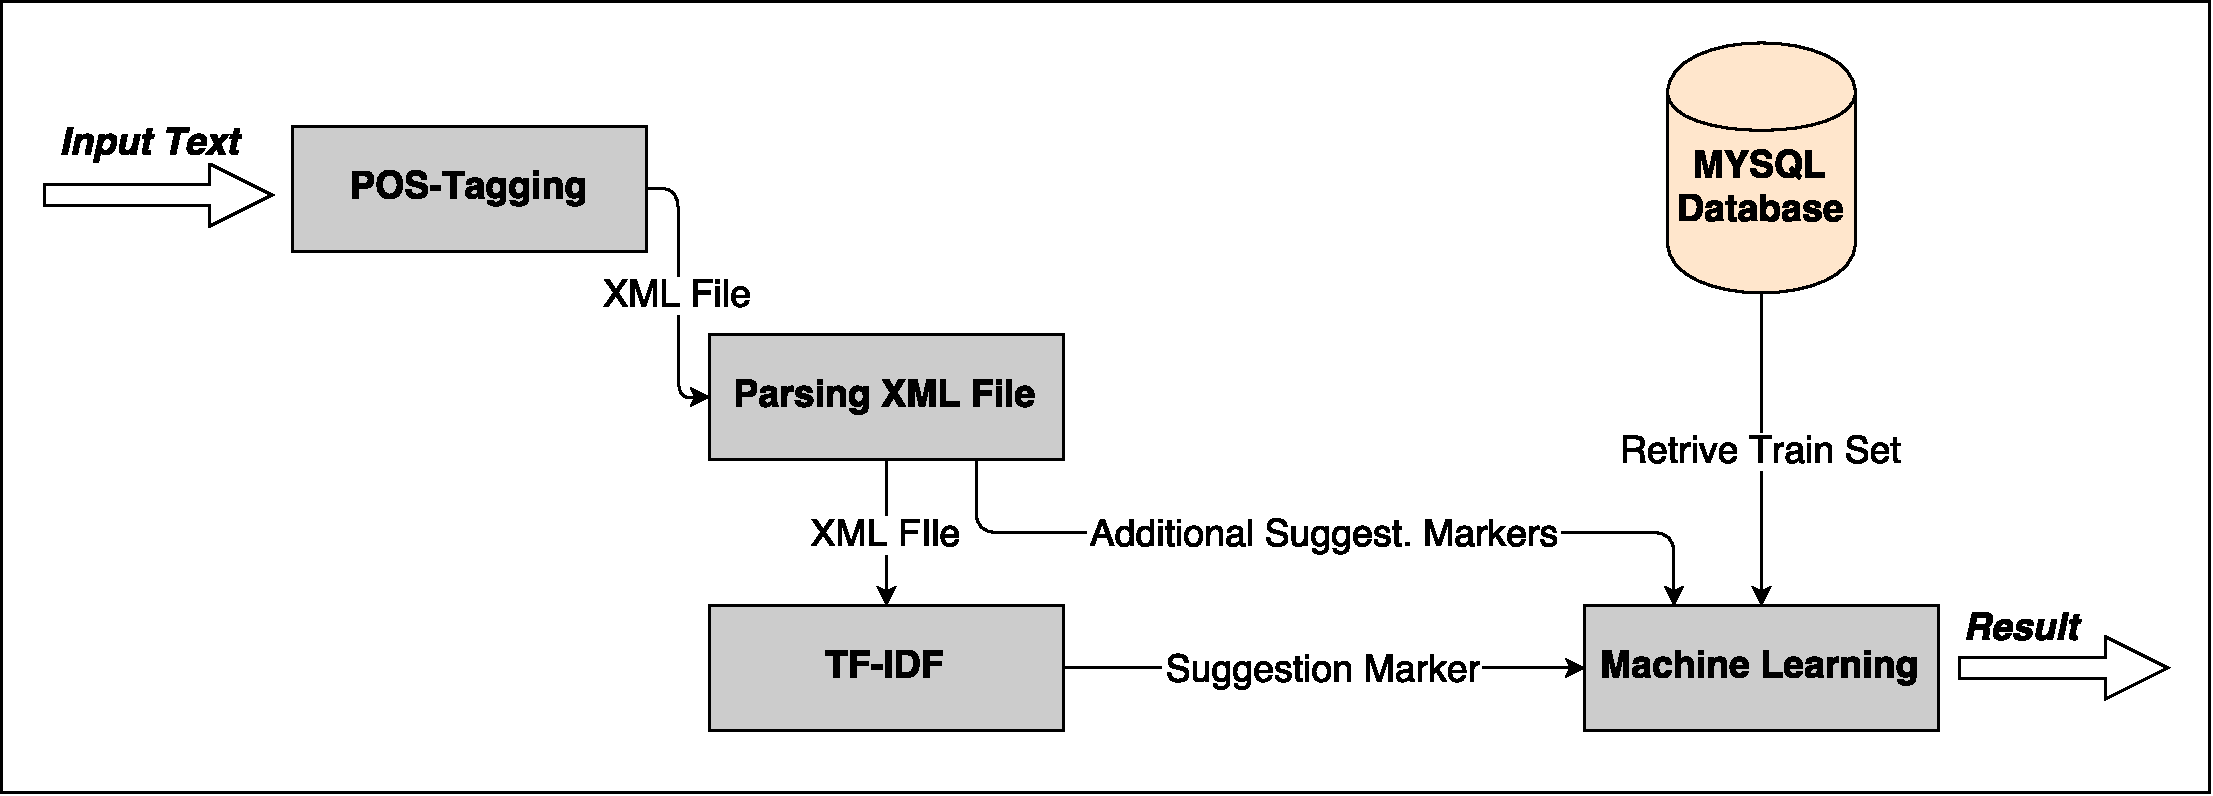
\includegraphics[width=1\linewidth]{figure/methods/suggestion_extraction.pdf}
\caption{Suggestion Extraction Process}
\end{figure}

Each one of the above steps will be explained in detail, in the next sections.

\subsection{Selecting Suggestion Markers}\label{331_ref}
As in the previous chapter we have, at this stage, to set some suggestion markers i.e., some characteristics in each sentence, which, if they appear, then the sentence that is being studied probably contains a suggestion.\\
\\
The basic idea that we applied is based, to a great extent, on Greek Grammar. We found that a suggestion can be ``modelled'' better than an argument. The basic concept is that in order to make a suggestion, a writer is ``obliged'' to follow some grammatical rules.\\
\\
We know that according to Greek Grammar, in order to express incitement in a sentence, the writer should use mainly either the Imperative or the Subjunctive Grammatical mood. These two Grammatical moods are often linked to the meaning we want to detect in our texts.\\
\\
Starting with the aforementioned concept, we noted that the use exclusively of Greek Grammar is not enough. In some way, we had to specify with more clarity what we were looking for in a text.\\
\\
\textbf{So, we extended the above concept. We combined Grammar rules with lemmas in order to achieve higher accuracy.}\\
\\
To make the above process clearer: Initially, using the ``ILSP POS-Tagger'' output, we noted the Grammar tags (\ref{3222_ref}), as well as the lemmas of verbs (\ref{3222_ref}) in order to create a list of verbs that are involved in cases where a sentence can be considered  as a suggestion. We can say that we noted the verbs which define the meaning of a sentence, making it a suggestion.\\
\\
An example can make the concept that was presented even clearer: Given the sentence \textit{``a change in paragraph 5 of the law  must be made..''} we noted that, in this example, ``must be made'' plays a determining role in order to put across the meaning of the sentence as a suggestion. This particular part of the sentence also has a particular Grammatical form.\\
\newpage
\lstset{language=XML,
  morekeywords={id,word,lemma,tag}
}
\begin{lstlisting}[frame=single, basicstyle=\small]
<?xml version='1.0' encoding='UTF-8'?>
<cesDoc xmlns="http://www.xces.org/schema/2003" version="0.4">
  <text>
    <body>
      <p id="p1">
        <s id="s1" casing="lowercase">
          <t id="t1" word="..." tag="VbIsIdPr03SgXxIpAvXx" lemma="..."/>
          <t id="t2" word="..." tag="PtSj" lemma="..."/>
          <t id="t3" word="..." tag="VbMnIdXx03SgXxPePvXx" lemma="..."/>
          <t id="t4" word="..." tag="NoCmFeSgNm" lemma="..."/>
          <t id="t5" word="..." tag="AsPpPaFeSgAc" lemma="..."/>
          <t id="t6" word="..." tag="NoCmFeSgAc" lemma="..."/>
          <t id="t7" word="..." tag="DIG" lemma="..."/>
          <t id="t8" word="..." tag="AtDfMaSgGe" lemma="..."/>
          <t id="t9" word="..." tag="NoCmMaSgGe" lemma="..."/>
          <t id="t10" word="..." tag="PTERM_P" lemma="..."/>
        </s>
      </p>
    </body>
  </text>
</cesDoc>
\end{lstlisting}

More precisely, we noticed that some tags, such as ``VbLsLdPr03SgXxLpAvXx'' and ``VbMnLdXx03SgXxPePvXx'' appear in many cases. Finally, we created a list with many cases that we detected. Some cases appear below:\\

\begin{itemize}

	\item We have to VbLsLdPr03SgXxpAvXx PtSj
	\item PtSj VbMnLdXxPepvXx must be studied
	\item VbMnLdXx03SgXxPePvXx PtSj must be applied
	\item Add PtSj VbMnLdPr03SXxLpPvxX
	\item ...\\

\end{itemize}
The above list is, in essence, the suggestion markers that we created. (The full list contains about eighty suggestion markers. The list is part of the submitted code.) Also some information about the POS-Tagger tagset can be found in section (\ref{3222_ref}).

\subsection{POS-Tagging and Lemmatization of the set of Documents}\label{332_ref}
The second stage for suggestion mining lies in the POS-Tagger performance. This process is the same as the one described in unit (\ref{322_ref}) and for the sake of brevity it will not be analysed again here.

\subsection{Apply Information Retrieval Methods in order to find the Suggestions}\label{333_ref}
Having created the suggestion markers, as we saw in subsection (\ref{321_ref}), we have, at this point, to analyse the way with which we can find similarities between the sentences being analysed and the suggestion markers.\\
\\
Initially, for every sentence in the process of analysis, the POS-Tagging \& Lemmatization method (\ref{332_ref}) is applied. From the Output of this process we make good use of the information that is absolutely essential for this step. So, for every sentence we keep the following information:\\
\begin{itemize}

	\item the verb tag.
	\item the verb lemma.
	\item the lemmas of words ``to'', ``will''.
	\item tags of the words ``to'', ``will''.
	\item ``Qst'' if the sentence is interrogative.\\

\end{itemize}

So, the sentence that we saw above, \textit{``a change must be made''} in paragraph 5 of the law'' becomes \textit{``VbLsLdPr03SgXxLpAvXx should PtSj be VbMnLdXx03SgXxPePvXx made''}.\\
\\
The next step is to create a similarity score between the sentence that came up and each one of the suggestion markers. The comparison was made using TF-IDF\footnote{\url{https://en.wikipedia.org/wiki/Tf\%E2\%80\%93idf}} and Jaccard Similarity\footnote{\url{https://en.wikipedia.org/wiki/Jaccard_index}} and as we will see in the following subsection, the results were satisfying enough.\\
\\
One more point that we need to stress is that we divided the suggestion markers in 4 categories, depending on the Grammatical mood, ``Imperative'' or ``Subjunctive'' and depending on whether the verbs are in a Past Tense (should have). The categories, as well as all the suggestion markers can be found in the ``suggestionQ'' folder through the online repository\footnote{\url{https://github.com/csdRepo/OpinionMining.git}}.\\
\\
Finally, having made the above comparisons, only the highest score will be kept, as well as the category from which this score came up. We should also note that the sentences that contain ``Qst'' automatically get zero score because we wanted to exclude the interrogative sentences for the same reasons that were mentioned earlier.

\subsection{Additional features for the optimization of Machine Learning Processs}\label{334_ref}
In order to achieve better results in each sentence that resulted from the above process, we counted the number of words from which it is made up.

\subsection{Apply Machine Learning}\label{335_ref}
The last stage for the retrieval of suggestions is the application of a Machine Learning Process. To implement this process, a train set and a test set must be definitely determined.

\subsubsection{Selecting Train and Test Set}\label{3351_ref}
In this case the train set is stored in the Database. To be precise, the retrieval of the train set from the Database is done with the following query:\\
%\newpage
\lstset{language=SQL}
\begin{lstlisting}[frame=single, basicstyle=\small]
SELECT
	opngv_suggestion.weight,
	opngv_suggestion.category,
	opngv_suggestion.total_words,
	opngv_trainset.Suggestion
FROM
	opngv_sentence
	INNER JOIN opngv_suggestion
		ON opngv_sentence.comment_id = opngv_suggestion.comment_id
		AND opngv_sentence.sentence_id = opngv_suggestion.sentence_id
	INNER JOIN opngv_trainset
		ON opngv_sentence.comment_id = opngv_trainset.comment_id
		AND opngv_sentence.sentence_id = opngv_trainset.sentence_id
ORDER BY
	opngv_trainset.Suggestion DESC
LIMIT 366
\end{lstlisting}

In this case, too, the test set consists of the sentences of the text, more precisely, the sentences that came up from the process (\ref{333_ref}).

\subsubsection{Machine Learning Process}\label{3352_ref}
As in the Argument Extraction (\ref{3232_ref}), the Weka Framework was also used here. Again, for the sake of brevity, it will not be analysed here.

\subsubsection{Machine Learning Algorithms}\label{3353_ref}
To verify the accuracy of the Train Set,we tested enough Algorithms:\\

\begin{itemize}

		\item Native Bayes\footnote{\url{https://en.wikipedia.org/wiki/Naive_Bayes_classifier}}
	\item Support Vector Machines\footnote{\url{https://en.wikipedia.org/wiki/Support_vector_machine}}
	\item Random Forest\footnote{\url{https://en.wikipedia.org/wiki/Random_forest}}
	\item J48\footnote{\url{https://en.wikipedia.org/wiki/J48}}

\end{itemize}

\section{Overall Opinion Extraction}\label{34_ref}
In this final chapter, the third leg of this Thesis, where the possibility of recognising the general degree of the writer's agreement with regards to the initial public consultation text of the Greek Government was studied, will be analysed. For this process, no kind of meta-data which would have supplied this information automatically (Agree/Disagree button, Like etc.), was used. The whole process has been completed by studying exclusively the users' texts.\\
\\
For the effective mining of this kind of information from the texts, we used the ``Sentiment Analysis'' method, in an attempt to recognise the sentiments with which the users write their texts. Having analysed the sentiments, we noted that very often it seems that they match each writer's degree of agreement. In more detail, this process can be divided as follows:\\
\begin{itemize}

	\item Translate Documents to English (\ref{341_ref}).
	\item Perform Sentiment Analysis  (\ref{342_ref}).\\

\end{itemize}

\begin{figure}[H]
\centering
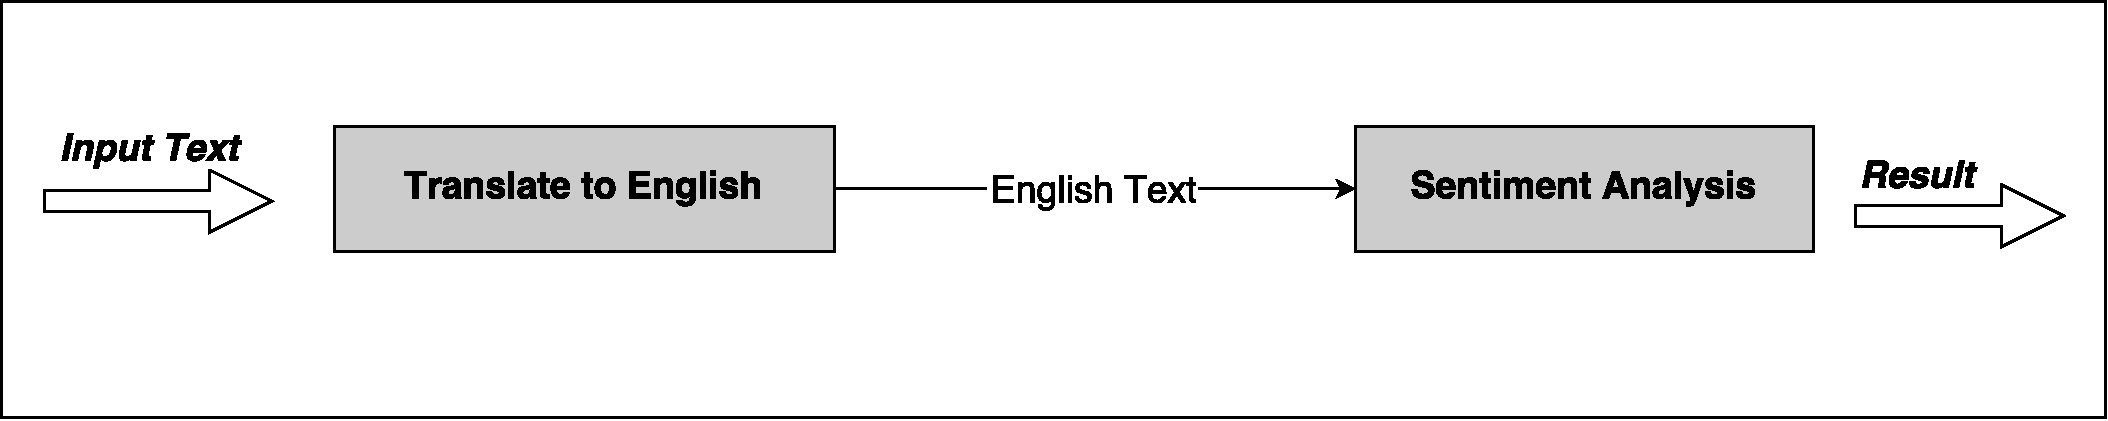
\includegraphics[width=1\linewidth]{figure/methods/overall_extraction.pdf}
\caption{Suggestion Extraction Process}
\end{figure}

\subsection{Translate Documents to English}\label{341_ref}
In order to be able to perform Sentiment Analysis, we had, in the first stage, to automatically translate the texts in the English language. The reason is that all the tools that are available do not support the Greek language. Also, studying and developing software that could perform Sentiment Analysis for Greek could constitute an independent task.\\
\\
It makes sense to think that with automatic translation, there are many times where the meaning of a sentence is altered and the translated text has many mistakes. This problem is even greater in Greek, because it has a complex and rich Grammar and subsequently, the texts in this case may be even more altered.\\
\\
Nevertheless, the above alterations do not affect the application of Sentiment Analysis. This happens because during Sentiment Analysis implementation, we are more interested in the connotation of the words, i.e. how much of a negative or positive meaning a word gives to a text.\\
\\
For the automatic translation of texts  from Greek to English, ``Google Translate'' has been used, a service provided for free through the appropriate API\footnote{\url{https://cloud.google.com/translate/}}.
\subsection{Perform Sentiment Analysis}\label{342_ref}
In the demo that accompanies this Thesis, there is the possibility to use two external tools that provide this kind of option.\\
\begin{itemize}
	\item
	 \textbf{SentiStrength\footnote{\url{http://sentistrength.wlv.ac.uk}}:}
	 \textit{“SentiStrength estimates the strength of positive and negative sentiment in short texts, even for informal language. It has human-level accuracy for short social web texts in English, except political texts. SentiStrength reports two sentiment strengths:}\\

	\begin{itemize}
		\item \textit{-1 (not negative) to -5 (extremely negative)}
		\item \textit{1 (not positive) to 5 (extremely positive)}\\
	\end{itemize}


\textit{Why does it use two scores? Because research from psychology has revealed that we process positive and negative sentiment in parallel - hence mixed emotions.
SentiStrength can also report binary (positive/negative), trinary (positive/negative/neutral) and single scale (-4 to +4) results.”}\\

	\item
	\textbf{Sentiment Analysis with Python NLTK Text Classification\footnote{\url{http://text-processing.com/docs/sentiment.html}}:} 
	\textit{“Sentiment analysis using a NLTK 2.0.4 powered text classification process. It can tell you whether it thinks the text you enter below expresses positive sentiment, negative sentiment, or if it's neutral. Using hierarchical classification, neutrality is determined first, and sentiment polarity is determined second, but only if the text is not neutral.”}
\end{itemize}









